\section{Overview}

This chapter describes the system design and presents the methodology
used to design and develop the project while achieving the objectives of
the study. It outlines the complete workflow of the project, starting
from the system concept and design requirements, through hardware and
firmware development, PCB design and manufacturing, and finally to
system deployment. The chapter also describes the calibration and
validation of the selected soil moisture sensor in comparison with
professional-class sensors.

\section{System Concept and Design
Requirements}

\subsection{System Concept}

The system is designed as a wireless mesh network using LoRa as the core
communication technology. Weatherproof wireless sensor nodes collect
data such as soil moisture, soil temperature, air humidity, and air
temperature, and transmit this data efficiently between neighboring
nodes until it reaches a base station with access to a cloud database.
The collected data is then made accessible to researchers from anywhere.

\begin{figure}[htbp]
\centering
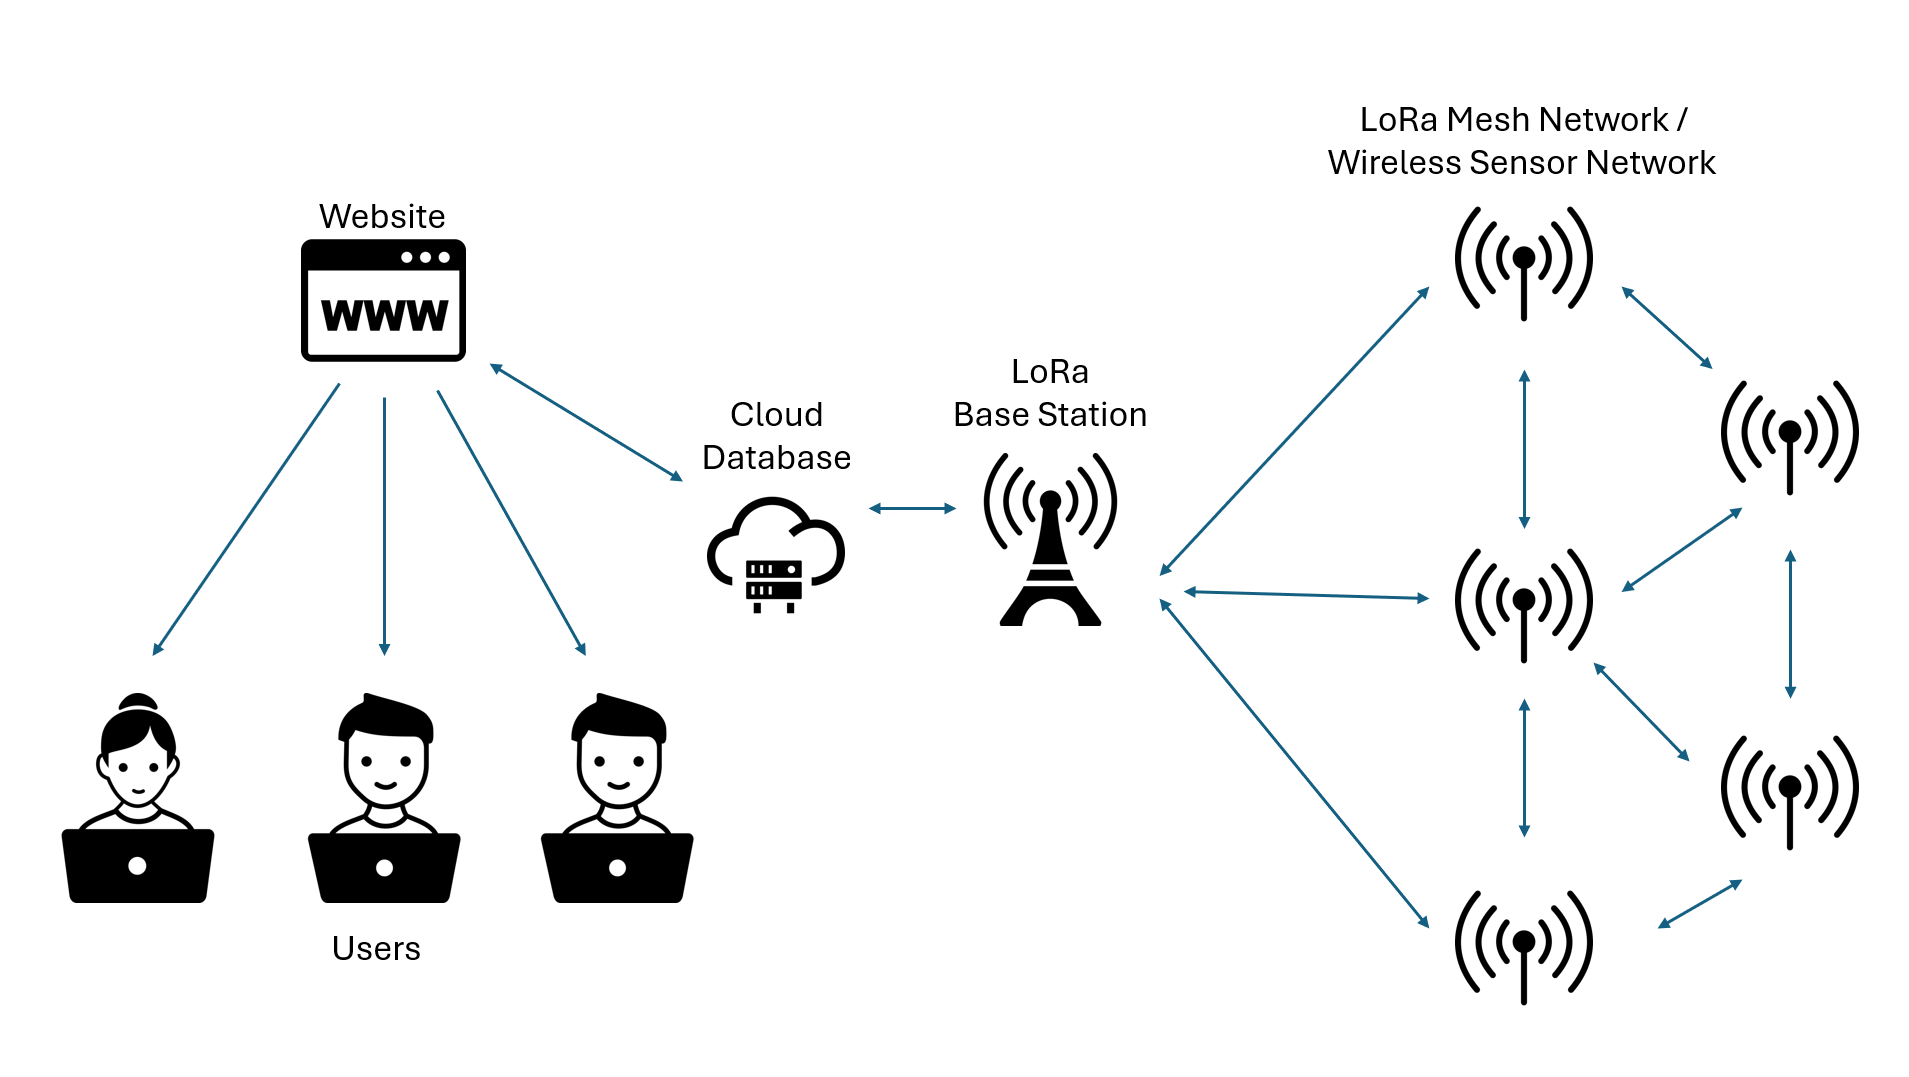
\includegraphics[width=5.03874in,height=2.8429in]{figs/method-image1.png}
\caption{Your figure description}
\label{fig:method-image1}
\end{figure}

LoRa was selected for its effectiveness over the short to medium
distances between turf houses, with the mesh topology improving network
robustness.


\par

\subsection{Functional
Requirements}


Since turf houses are considered natural heritage sites and museums, the
system must be invisible to visitors. Therefore, the sensor nodes must
be well hidden while still being effective in gathering data. The
functional requirements of the system are as follows:

\begin{itemize}
\item
  The sensor nodes must be capable of accurately measuring the required
  data, including soil moisture, soil temperature, air temperature, and
  air humidity.
\item
  The system must reliably transmit data through the mesh network, even
  with disturbances between nodes and the presence of noise.
\item
  The system must be able to operate for extended periods of time, as
  maintenance will be sparse due to the remote locations of turf houses.
\item
  The sensor nodes must be able to back up data to local storage in case
  of missed transmissions.
\item
  The collected data must be uploaded to a cloud network where it can be
  accessed and analyzed by researchers from anywhere.
\end{itemize}

\subsection{Environmental and Design
Constraints}


Multiple design constraints were identified following discussions with
experts in soil moisture sensing and turf roof construction. These
discussions highlighted several environmental and design factors that
needed to be considered for the system. The identified constraints
include the following:


\begin{itemize}
\item
  Sensor nodes will be buried at depths of approximately 11 cm and may
  be covered by additional layers of snow during winter.
\item
  The device must be sufficiently weatherproof to withstand harsh
  Icelandic conditions, including high moisture levels from rain and
  exposure to repeated freezing and thawing cycles across seasons, as
  well as prolonged snow coverage.
\item
  The installation and overall design process must be non-destructive to
  preserve the turf roof and must remain visually unobtrusive in order
  to maintain the integrity of the heritage site.
\end{itemize}

\section{Hardware Design}

\subsection{In Situ Sensor}

The sensor nodes deployed beneath the turf roofs consist of a low-power
microcontroller unit (MCU), lithium-ion batteries, a real-time clock
(RTC) for synchronizing data collection with the main network, an SD
card for local data backup in case of missed transmissions, a soil
moisture sensor, a temperature and humidity sensor, and a LoRa module
for wireless communication.

Based on the scope of this project, low cost was one of the significant
factors considered during system design. As a result, the system is
primarily composed of off-the-shelf components that were carefully
selected based on their cost and performance. Power consumption was
another critical design consideration. To improve energy efficiency, all
components were selected to operate at 3.3 V or lower.

To further reduce power consumption, the design incorporates a
MOSFET-based power control system that disconnects power to sensors
while the system is in sleep mode. The sensor node is periodically
awakened by the real-time clock to collect, store, and transmit data
before returning to low-power sleep operation.

\begin{figure}[htbp]
\centering
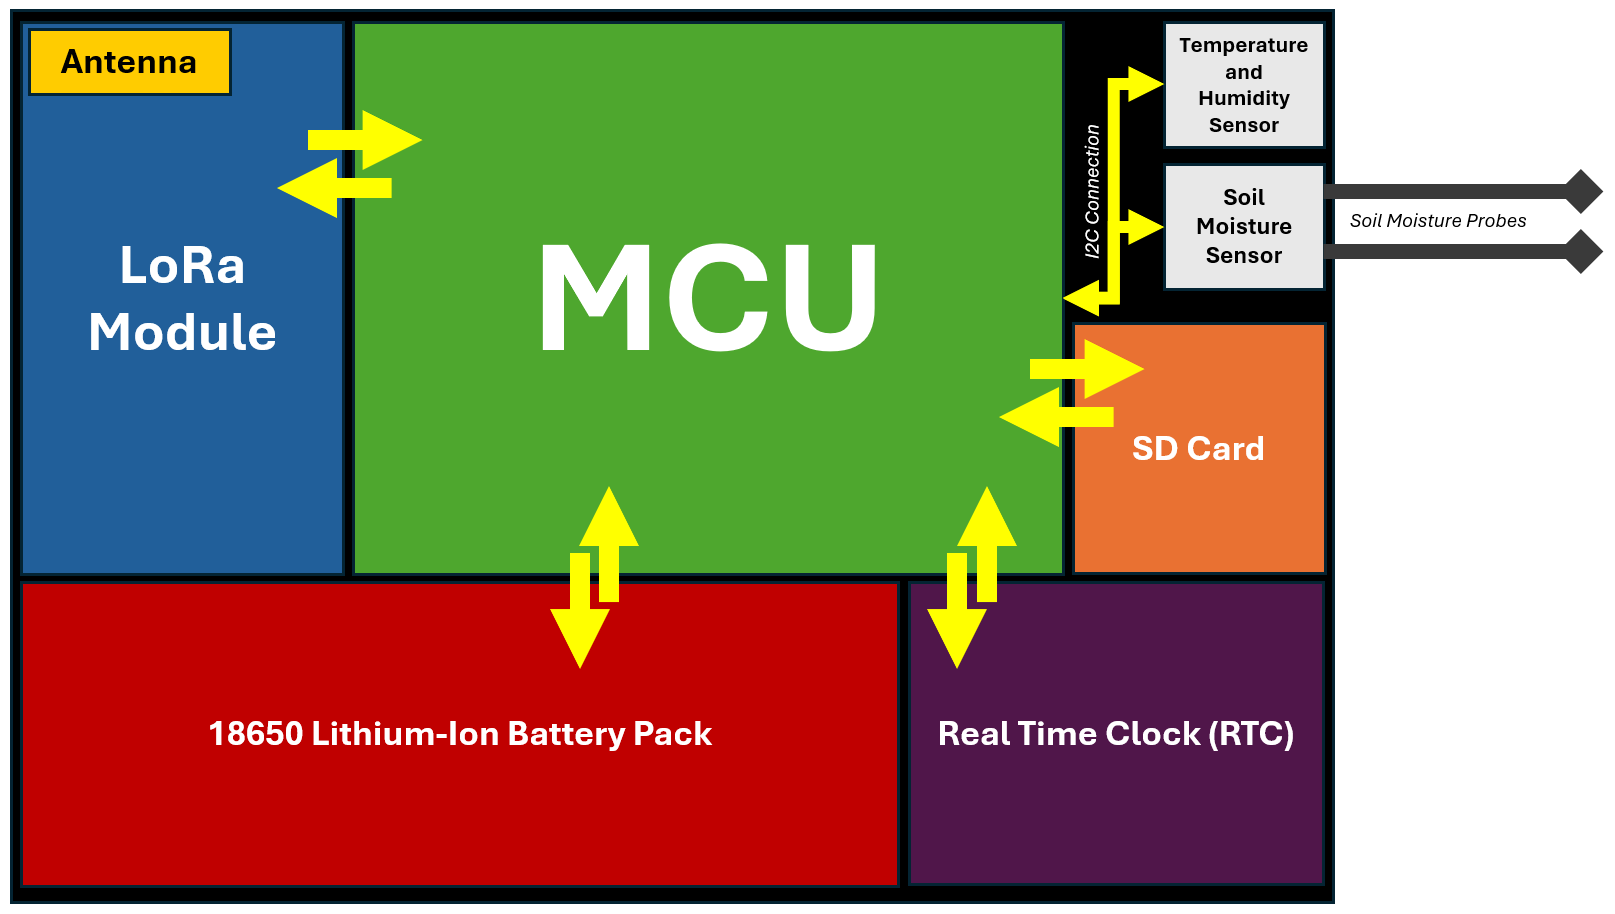
\includegraphics[width=5.48053in,height=3.10153in]{figs/method-image2.png}
\end{figure}

\subsubsection{Device Components}

\subsubsection{LoRa Module (Ra-02 SX1278
433Mhz)}

The Ra-02 LoRa module, based on the SX1278 transceiver,
operates at 433 MHz, which is within the legal ISM band in Iceland. The
module offers long-range communication capabilities of up to several
kilometers, which is more than sufficient for the expected distances
between turf houses. Additionally, the module has low power consumption
and a small physical footprint, making it suitable for a compact and
energy-efficient sensor node
design.


\subsubsection{Microcontroller (Arduino Pro
Mini)}

The choice of microcontroller was a critical design decision.
The microcontroller needed to be compact, energy efficient, and capable
of handling sensor data acquisition, storage, and wireless
communication. Several alternatives were considered, including the
ESP32; however, it was deemed unsuitable due to higher power
consumption, higher cost, and excess computational capability for the
requirements of this
project.


The Arduino Pro Mini, based on the ATmega328P
microcontroller, was selected as it operates at 3.3 V with an 8 MHz
clock frequency and provides 32 kB of flash memory. It supports both I2C
and serial communication, which are required for interfacing with the
sensors and peripheral modules. The available memory and processing
capability were found to be sufficient for the application. Power
consumption is approximately 4.5 mA during active operation and can be
reduced to approximately 3 µA in deep sleep mode after removing onboard
indicator LEDs, which was implemented in this
project.


\subsubsection{Air Temperature and Humidity Sensor
(AHT10)}

The AHT10 sensor was selected for measuring air temperature
and humidity due to its availability, low cost, and adequate accuracy
for the application. The sensor communicates via the I2C interface and
is capable of measuring temperatures from −40 °C to 85 °C with an
accuracy of ±0.3 °C. Relative humidity measurements range from 0\% to
100\% with an accuracy of ±2\%, which is sufficient for monitoring
environmental conditions beneath turf
roofs.


\subsubsection{Soil Temperature Sensor
(DS18B20)}

The DS18B20 digital temperature sensor was selected for soil
temperature measurements due to its simplicity, accuracy, and
robustness. The sensor operates over a temperature range of −55 °C to
125 °C with an accuracy of ±0.5 °C. It communicates using a one-wire
interface, requiring only three connections, which simplifies wiring and
reduces complexity. Waterproof probe-style versions of the DS18B20 are
widely available, making the sensor well suited for buried soil
applications.


\subsubsection{Soil Moisture Sensor (Capacitive Soil Moisture
Sensor
v1.2)}

A generic off-the-shelf capacitive soil moisture sensor (v1.2) was used
in this study. The sensor design is open source and widely available,
resulting in many similar commercial versions. This sensor outputs an
analog voltage that varies with the soil moisture content, which is read
by the Arduino as an analog value within the range defined by the 3.3 V
supply voltage. Despite being low cost, previous studies have shown that
capacitive soil moisture sensors can provide consistent and reliable
measurements when properly selected and calibrated, as discussed in
Chapter 2.

Capacitive sensors were chosen over resistance-based alternatives due to
their improved reliability and reduced susceptibility to corrosion in
moist soil environments. While professional-grade soil moisture
measurement methods such as TDR and FDR offer higher accuracy, they are
significantly more expensive and less suitable for large-scale
deployment. In contrast, low-cost capacitive sensors offer a practical
solution for distributed monitoring applications, such as turf roof
installations.

In this study, the selected sensor was used with the understanding that
calibration is required to improve measurement accuracy. By calibrating
the sensor against professional-grade reference instruments, the system
aims to achieve accurate soil moisture measurements while maintaining
low cost and scalability.

\subsubsection{SD Card Module (SparkFun OpenLog Serial
Logger)}

Local data storage was implemented using the SparkFun OpenLog
serial logger module. Several SD card modules were initially evaluated;
however, many were found to be too large, power intensive, or required
software libraries that exceeded the available flash memory of the main
microcontroller.


The OpenLog module records data received over a serial
interface directly to a microSD card and is based on its own ATmega328
microcontroller, allowing it to operate independently of the main MCU.
This approach significantly reduces memory usage on the sensor node. The
module supports microSD cards up to 32 GB and consumes approximately
2--6 mA during operation, making it suitable for low-power data
logging.


\subsubsection{Power Source (18650 Samsung 35E 3500mAh Li-Ion
Battery)}

The system is powered using three 18650 lithium-ion
batteries, each with a nominal capacity of 3500 mAh, providing a total
capacity of 10,500 mAh. These batteries operate over a voltage range of
approximately 2.65 V to 4.2 V, which is suitable for a 3.3 V
system.


To ensure safe operation within voltage limits, a Zener diode
is used to reduce the maximum input voltage by approximately 0.5 V. This
configuration ensures compatibility with the 3.3 V power requirements
while providing sufficient capacity for long-term
operation.


Size was an important consideration in the design of the sensor modules.
However, sourcing batteries with a small form factor and high capacity
was severely limited by import fees, availability, and cost. As a
result, a conventional and widely available 18650 lithium-ion battery
was selected.

\subsubsection{Real Time Clock
(DS3231)}

The DS3231 real-time clock was selected due to its high accuracy, low
power consumption, and integrated temperature-compensated crystal
oscillator. The module includes a battery backup and consumes
approximately 100 µA in standby mode. It supports up to two programmable
alarms capable of generating an interrupt signal, which is used to wake
the microcontroller from deep sleep mode.

This functionality is critical for synchronizing sensor nodes and
ensuring consistent data collection and transmission intervals across
the mesh network.

\subsubsection{Antenna (433Mhz
3dbi)}

The selected antenna operates at 433 MHz, which matches the
configuration of the system. The antenna has a minimal design and is
commonly used for radio communication applications, making it suitable
for LoRa operation. Although the antenna has a gain of only 3 dBi, it
provides significantly better performance than operating without an
external antenna.

Additionally, the antenna's compact and discreet design allows it to
blend well with the surrounding environment. Its small size and vertical
form factor make it visually unobtrusive, resembling tall grass, which
is important for maintaining the stealth and aesthetic requirements of
the turf roof installation.

\subsubsection{Schematic Design}

This section describes the schematic design of the main
printed circuit board (PCB) used for the sensor node. To compactly
integrate all components into the smallest possible form factor and to
simplify assembly and wiring, a custom PCB was designed and
manufactured. The PCB houses all system components described in the
previous section, with the exception of the batteries, along with
additional circuitry required for system
functionality.


\subsubsection{\begin{figure}[htbp]
\centering
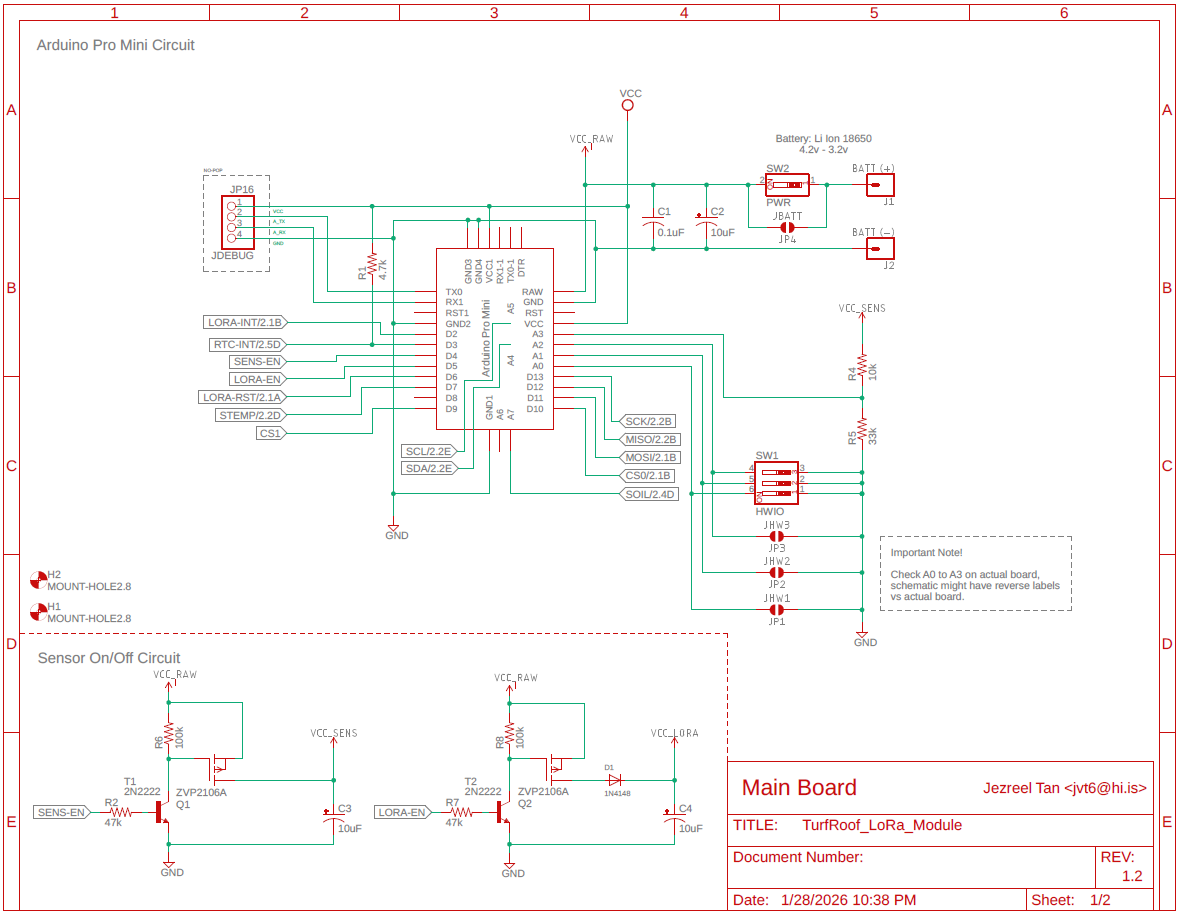
\includegraphics[width=5.43347in,height=4.22139in]{figs/method-image3.png}
\end{figure}}

Battery voltage monitoring is implemented using a simple voltage divider
connected to analog pin A3 of the microcontroller. The microcontroller
reads the divided voltage as an analog value, which is then converted
back to the corresponding battery voltage in software. This allows the
system to monitor battery health during operation.

To minimize power consumption during sleep periods, the design includes
MOSFET-based power control for two sensor groups, labeled SENS-EN and
LORA-EN. When the system enters deep sleep mode between data collection
intervals, the microcontroller disables both MOSFETs, effectively
cutting power to the sensors and the LoRa module. Each group is only
powered when required and is turned off immediately afterward, ensuring
minimal power consumption during inactive periods.

\subsubsection{Hardware ID}

As shown in the schematic, the core of the board is the Arduino Pro Mini
microcontroller. A component labeled SW1 is used as a three-bit hardware
identifier, allowing each sensor node to be assigned a unique ID. Upon
boot, the microcontroller reads the state of these bits and assigns the
corresponding hardware ID to the node, preventing data collisions during
transmission. With this configuration, up to seven unique devices can be
supported within a single system. The design can be further scaled by
adding additional identifier bits using available microcontroller pins.
For deployments involving multiple systems, software-based hardware
prefixes can be implemented to distinguish between different system
groups.

\begin{figure}[htbp]
\centering
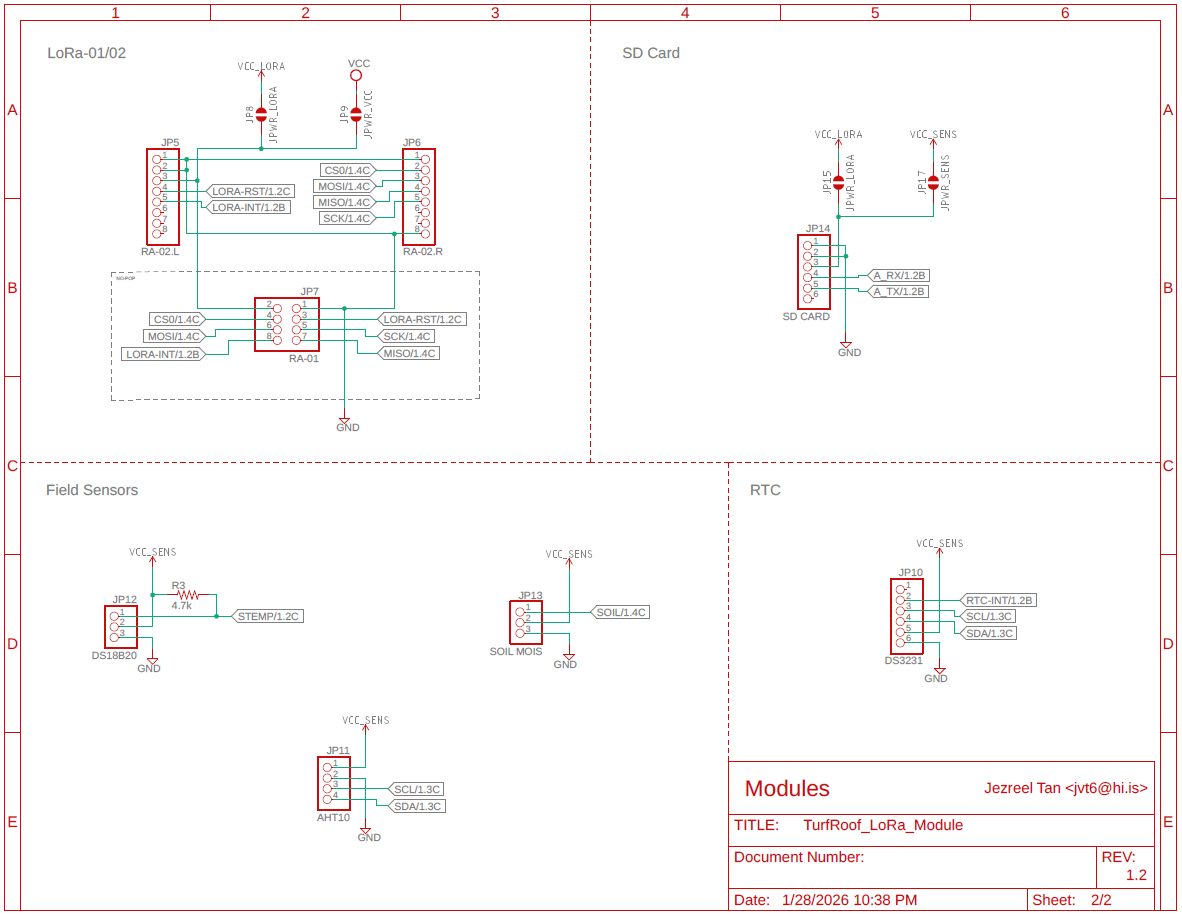
\includegraphics[width=5.59929in,height=4.33885in]{figs/method-image4.png}
\end{figure}

The PCB layout was primarily designed to accommodate the Ra-02 LoRa
module. However, based on feedback from users with experience in LoRa
systems, an alternative module package (Ra-01), which offers similar
specifications but a different form factor, was also considered. To
support this flexibility, a no-populate drop-in footprint was included
on the PCB, allowing either module to be used depending on availability
or user preference.

For the sensor interfaces, pin headers were used to simplify the design,
testing, and development process. This approach allows sensors to be
easily connected and disconnected, improving ease of assembly and
enabling quicker replacement or modification during testing and
deployment.

\subsubsection{PCB Design and
Manufacturing}

During the PCB design process, cost and compactness were carefully
considered. The main PCB for a single sensor module was designed to fit
within a 50.5 mm × 50.5 mm footprint using a two-layer, 1.6 mm thick
FR-4 substrate. A two-layer design was sufficient due to the relatively
low routing complexity, helping to reduce manufacturing costs.

The PCB was manufactured by JLCPCB. Ground planes were incorporated
where possible to improve signal integrity and reduce noise,
particularly around the LoRa transceiver. Component placement was
optimized to allow ease of manual assembly and debugging during
development.

The use of pin headers for the sensors simplified the assembly process,
allowing sensors to be rearranged easily and packed neatly within the
enclosure.

\begin{figure}[htbp]
\centering
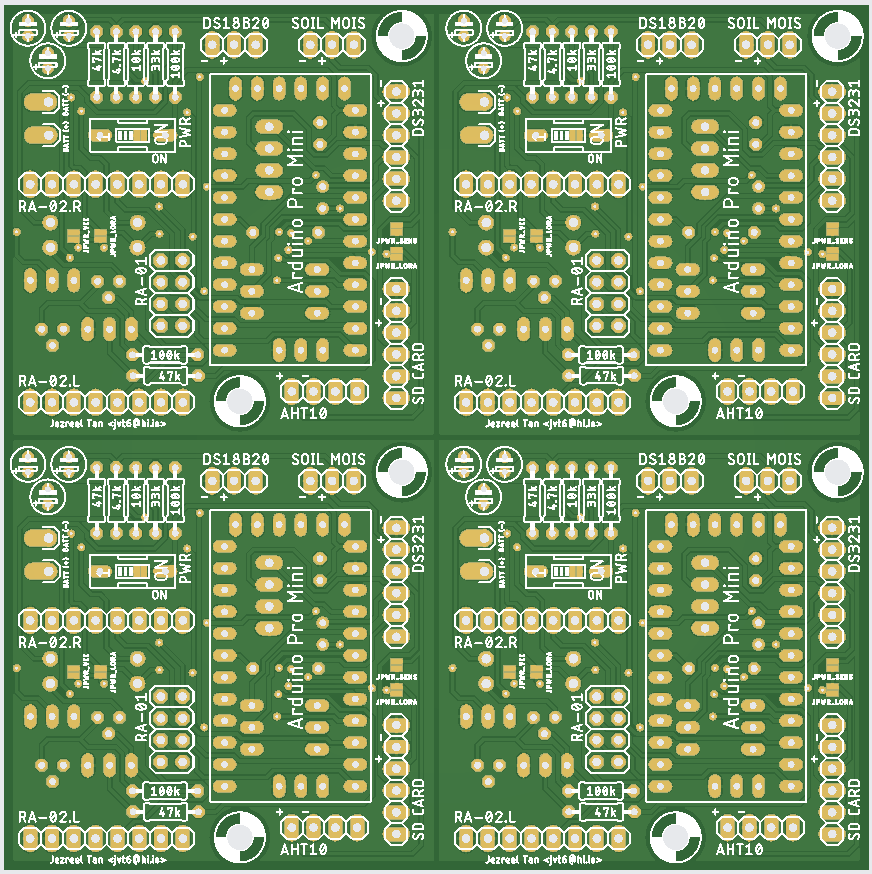
\includegraphics[width=3.84123in,height=3.84985in]{figs/method-image5.png}
\end{figure}

\subsubsection{System Assembly}

To ensure reliable operation under the harsh environmental conditions in
Iceland, all sensor components were enclosed in a weatherproof and
waterproof housing. The components were assembled neatly inside the
enclosure to protect them from moisture, rain, snow, and temperature
variations. Although the initial goal was to minimize the size of the
sensor module---ideally approaching the size of the main PCB---the
batteries were the primary limiting factor in reducing the overall form
factor. Nevertheless, the final design remained compact, easy to handle,
and capable of housing sufficient battery capacity for long-term
operation.

Two enclosure designs were developed and evaluated to determine which
configuration provided better performance and practicality. The first
design integrated the LoRa antenna directly into the main sensor
enclosure. This resulted in a more compact and mechanically robust
module with fewer loose components. However, this configuration limited
flexibility during installation, particularly in confined or uneven
mounting locations.

The second design utilized an external waterproof enclosure connected
via a cable, housing both the LoRa antenna and the AHT10 air temperature
and humidity sensor. This configuration allowed the air sensor to be
positioned above ground, resulting in more representative air
temperature and humidity measurements. However, this design increased
exposure of the sensor and cabling to environmental elements, requiring
additional protection to prevent potential damage.

After assembly, all seams, cable entry points, and enclosure openings
were sealed using silicone sealant to ensure watertightness. This final
sealing step was critical in protecting the electronics from water
ingress caused by rain, snow, and meltwater, thereby improving the
overall durability and reliability of the system.

\begin{figure}[htbp]
\centering
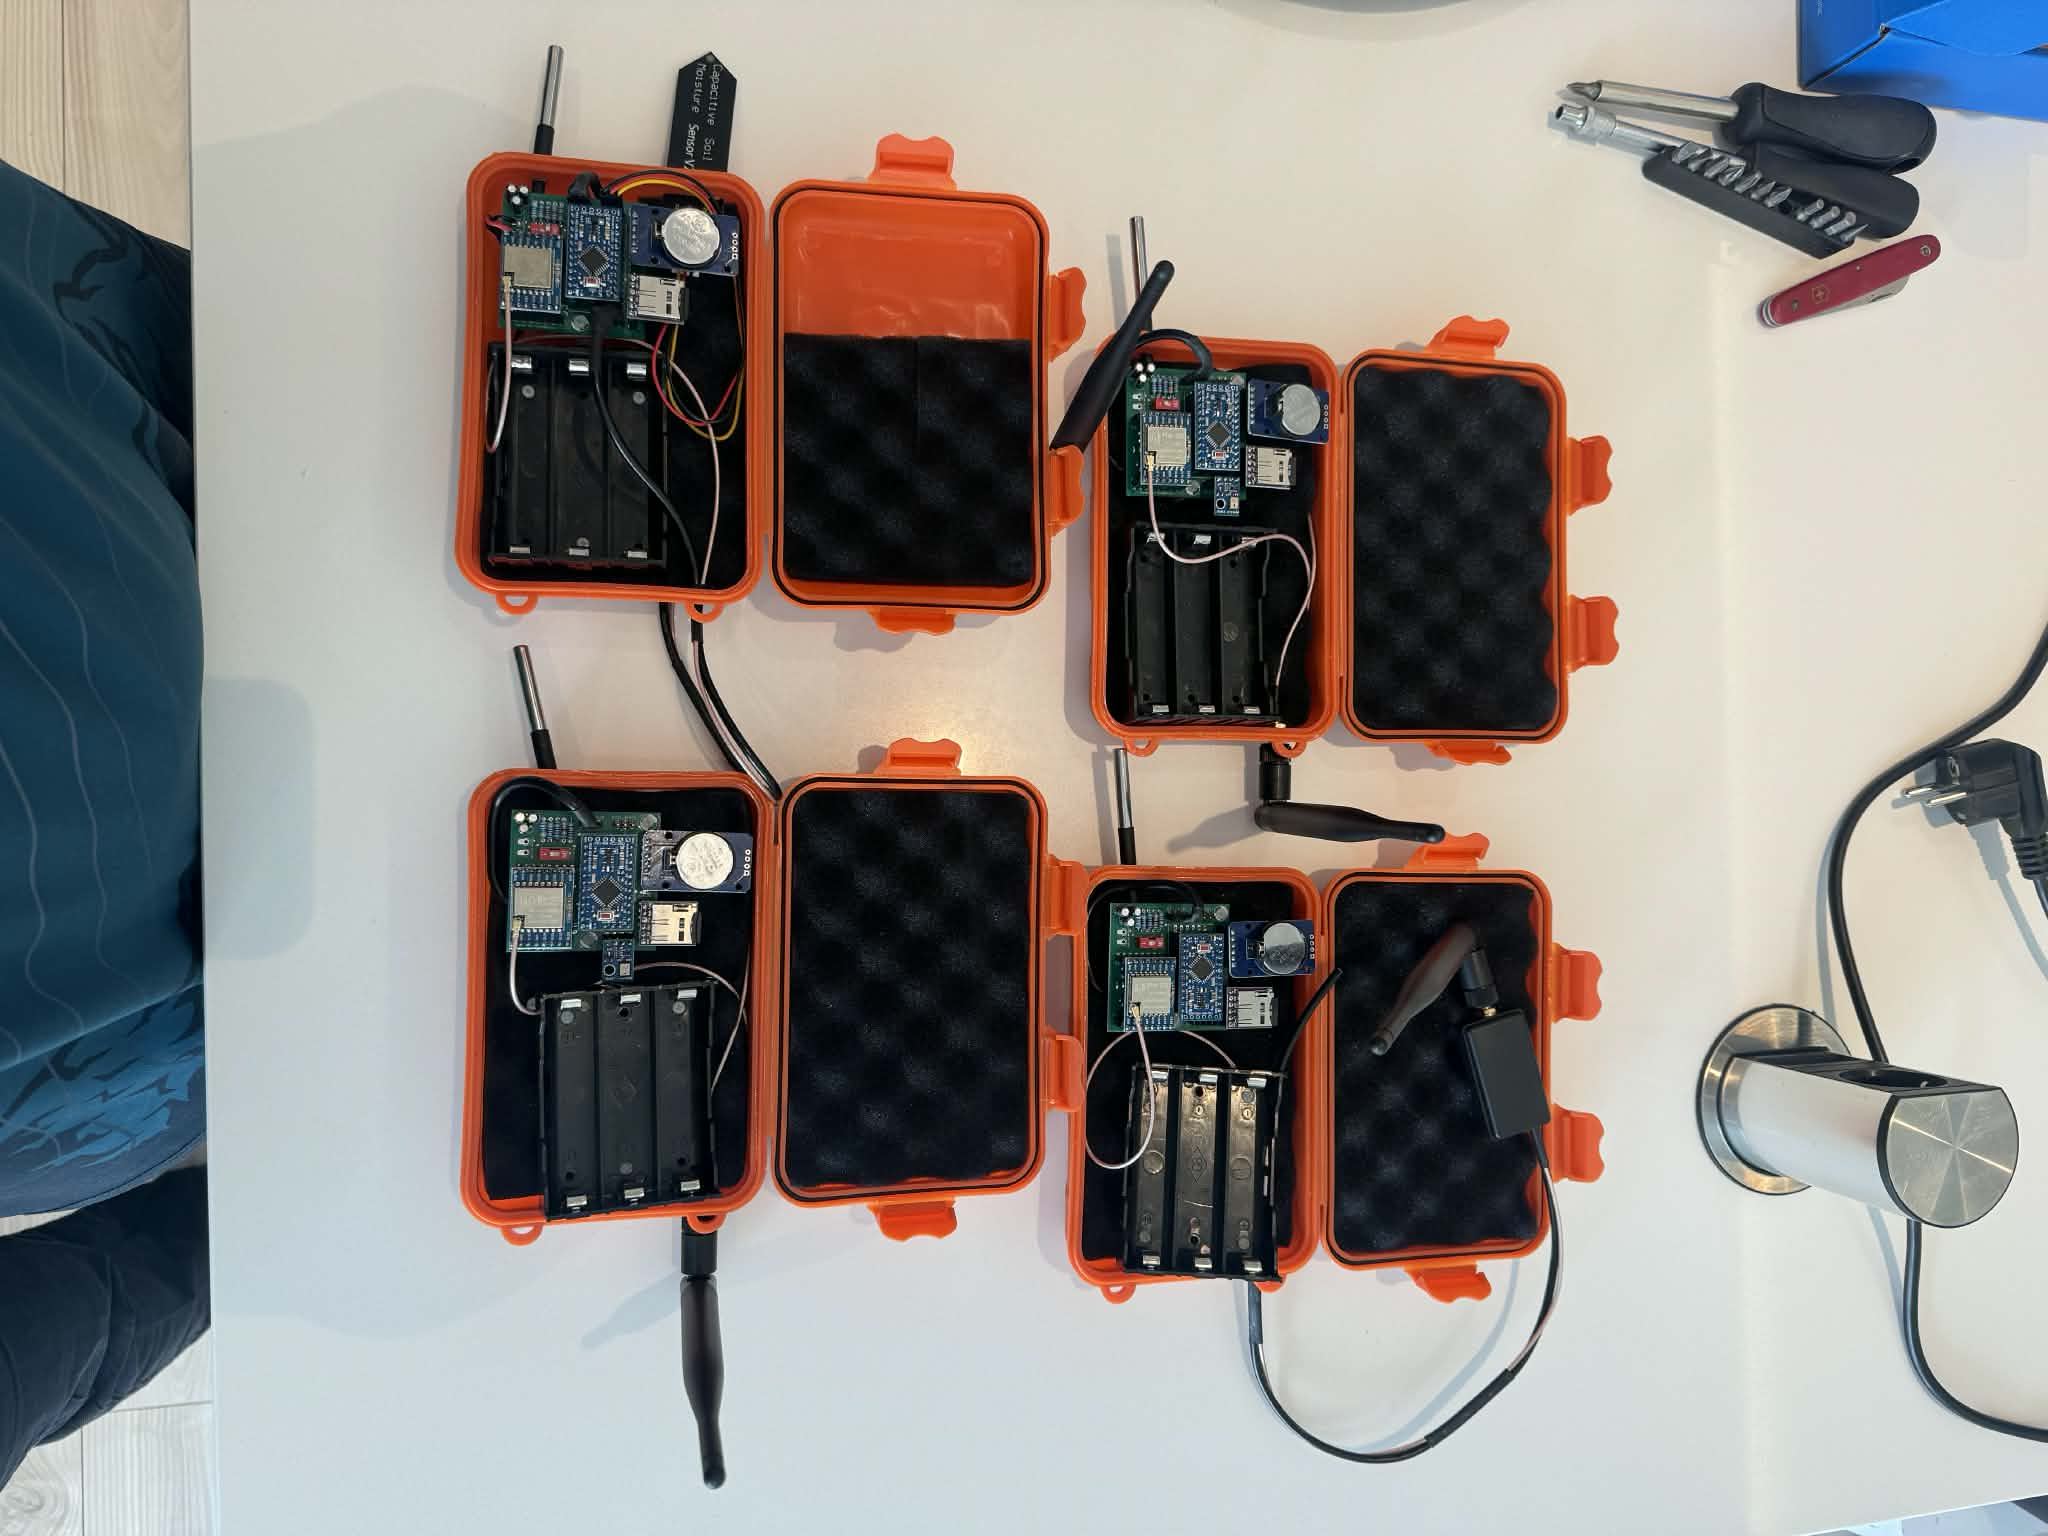
\includegraphics[width=4.33694in,height=3.25921in]{figs/method-image6.jpeg}
\end{figure}

\subsection{Base Station Module}

The base station module consists of a low-power microcontroller unit
(MCU) and a LoRa module. The MCU connects directly to the internet via
Wi-Fi to synchronize time and is powered through a mains outlet to
ensure a stable and continuous power supply. Using its internal clock,
the MCU enters sleep mode between intervals and periodically checks the
time through the internet to ensure accurate wake-up timing.

At scheduled intervals, the base station MCU sends a signal to all
sensor nodes to initiate data collection. At this time, all sensor nodes
are expected to be awake and ready to transmit data. Once the base
station receives all required data, it broadcasts the current date and
time to ensure that all sensor nodes remain time-synchronized. This
process allows the sensor nodes to be synchronized on an hourly basis.

After synchronization, the base station uploads the collected data to
the cloud, where it is stored and made available for viewing and further
data analysis by researchers.

\begin{figure}[htbp]
\centering
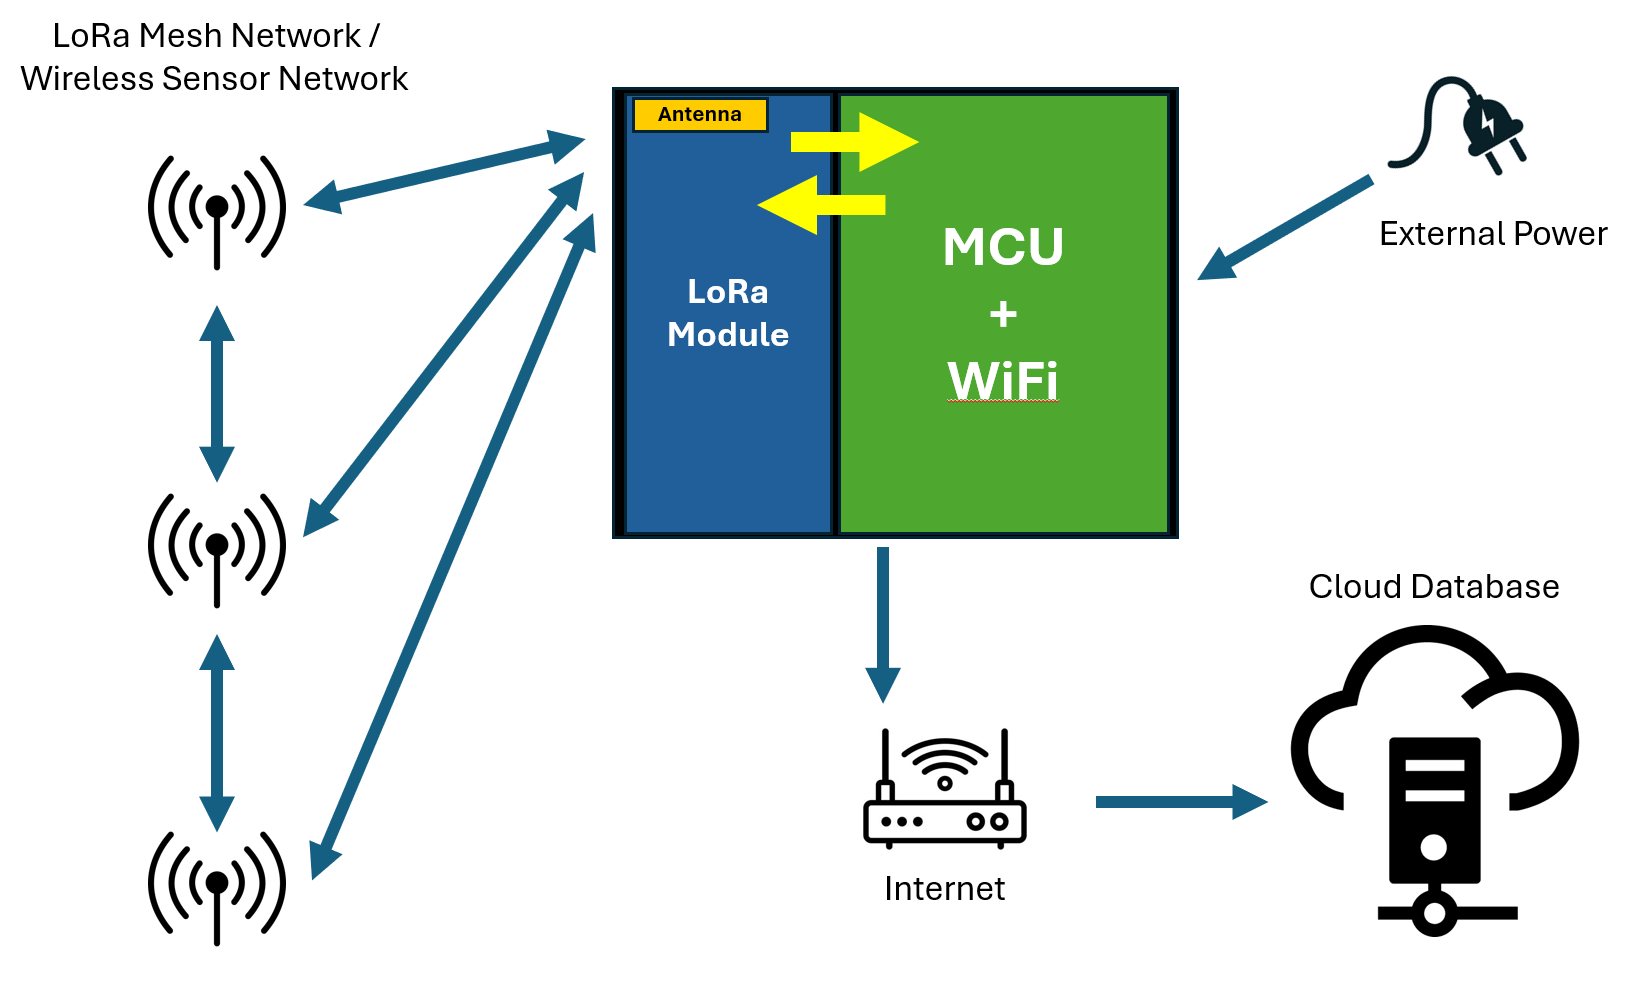
\includegraphics[width=\textwidth]{figs/method-image7.png}
\end{figure}

\subsubsection{Device Components}

\subsubsection{LoRa Module (Ra-02 SX1278
433Mhz)}

The base station uses the same Ra-02 LoRa module as the
in-situ sensor nodes to maintain consistency across the system. Using
the same LoRa module simplifies system design, firmware development, and
communication compatibility between the base station and sensor nodes.
Additionally, this approach reduces component variation and ensures
reliable and uniform communication performance throughout the
network.

\subsubsection{Microcontroller (LOLIN D1
mini)}


Initially, during the concept design and planning stage, a Raspberry Pi
was considered as the primary choice for the base station. Based on a
review of similar theses and related projects, many researchers used a
Raspberry Pi for comparable applications. However, after further
development and evaluation, it was concluded that a Raspberry Pi would
be excessive for the requirements of this system. In addition, it is
relatively costly, and several lower-power microcontroller-based
alternatives were found to be more suitable for the application.

Eventually, the LOLIN D1 mini was selected as the base station
controller. The board is based on the ESP8266EX chip, which provides
built-in Wi-Fi connectivity. It supports SPI communication, which is
required for interfacing with the LoRa module, and operates at 3.3 V
with an 80 MHz clock frequency and 4 MB of flash memory. These
specifications were sufficient for the data handling, communication, and
synchronization tasks of the base station. The board can be programmed
using C/C++, allowing efficient use of its limited flash memory and
providing flexibility for firmware customization. Additionally, the
module can be easily powered through a USB Type-C connection, enabling
the use of common power adapters for continuous operation.


\subsubsection{System Assembly}

The base station module has a relatively simple hardware configuration,
which made assembly and integration straightforward. Since both the
microcontroller and the LoRa module operate at 3.3 V, they can be
directly interconnected without the need for additional level-shifting
circuitry. The SPI communication lines were connected between the MCU
and the LoRa module, and the antenna was securely attached to the LoRa
module to ensure proper radio performance.

Power was supplied to the base station through a mains-powered adapter,
allowing continuous operation without power constraints. After assembly,
the microcontroller was programmed with the base station firmware, and
basic functionality was verified. Proper antenna installation was
ensured to avoid signal degradation during operation.

\section{Firmware}

The firmware for the proposed LoRa mesh wireless sensor network was
developed in C/C++ using an object-oriented programming (OOP) approach.
The system is based on the ATmega328P microcontroller, which is
well-supported within the Arduino development ecosystem and allows
efficient low-level hardware control. An object-oriented structure was
selected to improve modularity, scalability, and maintainability of the
system. By encapsulating functionality into separate classes (e.g.,
sensor handling, LoRa communication, data management, and power
control), the firmware becomes easier to debug, extend, and adapt for
future deployments or additional sensing requirements.

\begin{quote}
Firmware development and flashing were performed using the Arduino IDE.
Arduino was selected because of its open-source architecture,
comprehensive library support, and strong developer community, which
streamline firmware development, enable efficient debugging, and provide
flexibility for future system expansion. Standard Arduino libraries were
utilized where appropriate, including libraries for SPI communication
(LoRa module), I2C communication (environmental sensors), SD card
interfacing, and low-power sleep control. Custom logic was implemented
to manage mesh routing, data formatting, packet handling, and power
optimization.

Two primary firmware implementations were developed:
\end{quote}

\begin{enumerate}
\def\labelenumi{\arabic{enumi}.}
\item
  \textbf{In Situ Sensor Node Firmware} -- responsible for sensor data
  acquisition, packet formatting, mesh communication, local data backup,
  and low-power operation.
\item
  \textbf{Base Station Firmware} -- responsible for receiving and
  decoding mesh packets, managing acknowledgments, and uploading
  validated data to the cloud platform.
\end{enumerate}

\begin{quote}
The full source code repository is publicly available at:\\
\url{https://github.com/JezT25/turfroof_lora}
\end{quote}

\subsection{The LoRa Mesh System}

During the early stages of algorithm development, particular attention
was given to how sensor data could be distributed evenly, reliably, and
robustly across the mesh network. The primary objective was not only to
ensure that the base station received all measurements, but also to
enhance network resilience by reducing dependence on a single
communication path.

An architectural concept inspired by distributed ledger systems, such as
blockchain, influenced the final design. In blockchain systems, a shared
ledger acts as a synchronized and verifiable record of transactions
across multiple participants, ensuring consistency and integrity of
data. While the proposed system does not implement blockchain or
cryptographic consensus mechanisms, it adopts a simplified
distributed-ledger-inspired approach to improve robustness within the
LoRa mesh network.

In this implementation, the base station initializes a structured data
ledger template, which is propagated throughout the network. Each sensor
node appends its most recent measurement to the ledger before forwarding
it to neighboring nodes. Through multi-hop transmission, the ledger
circulates across the mesh until all participating nodes have
contributed their respective data entries.

This approach ensures that:

\begin{itemize}
\item
  Data redundancy is introduced at the network level.
\item
  Nodes can verify whether their measurements have been successfully
  incorporated.
\item
  The system reduces single points of failure.
\item
  Network robustness is improved in the event of intermittent
  connectivity.
\end{itemize}

By allowing all nodes to maintain awareness of the aggregated dataset
before final transmission to the base station, the system achieves
greater reliability compared to a traditional star topology where only
the base station holds the complete dataset. The final validated ledger
is then transmitted to the base station for cloud upload and long-term
storage.

\subsubsection{Architecture}

To simplify debugging and system validation during development, all LoRa
data packets were transmitted as human-readable plaintext strings.
Although this approach is less efficient than using compact binary
packet structures, it significantly improved transparency during early
testing and troubleshooting. Being able to directly inspect transmitted
data without additional decoding tools allowed for faster identification
of routing, formatting, and communication errors within the mesh
network.

It should be noted that, for a production-level implementation, a packed
data structure (e.g., a structured binary payload containing predefined
variables) would be preferable. Such an approach would reduce payload
size, improve transmission efficiency, and optimize airtime usage ---
particularly important in low-bandwidth LoRa systems.

The decision to retain plaintext transmission in the final prototype was
primarily influenced by the system's early testing phase, where
plaintext communication was initially implemented and validated.
Maintaining this format ensured consistency and stability throughout
development. Nevertheless, future iterations of the system would benefit
from migrating to a structured binary packet format for improved
scalability and performance.

3.4.1.1.1 The Packets

To initiate communication within the mesh network, one node ---
typically the base station --- broadcasts a structured ledger packet.
This ledger acts as a container for aggregated data and is circulated
among all participating nodes. The packet consists of three main
components: a header, reserved data fields for each node, and a checksum
value used for basic integrity verification.

Each node in the network is assigned a unique hardware ID. This ID
determines the fixed position within the packet where the node inserts
its data. For example, if a node has a hardware ID of 3, it writes its
measurement into the fourth allocated data field within the ledger. This
positional mapping prevents data overwriting and ensures deterministic
placement of measurements, allowing every node to know exactly where its
contribution belongs within the packet.

Because all data is transmitted in plaintext format, each node is
allocated a fixed number of characters. While a packed binary structure
with defined variable types would have been more memory-efficient and
flexible, fixed-width plaintext fields were chosen to simplify
debugging, inspection, and demonstration of the system. Each numerical
value is formatted to support a range from --99.9999 to 999.9999. This
range comfortably accommodates all measured parameters (e.g.,
temperature, humidity, soil moisture, battery voltage), ensuring no
overflow occurs within the defined field size.

To maintain low computational overhead on the ATmega328P
microcontroller, the checksum mechanism was intentionally simplified.
Instead of implementing a standard CRC16 or similar algorithm, the
checksum is computed as the arithmetic sum of numerical values from node
0 through node 7. While this does not provide the robustness of
industry-standard CRC implementations, it offers a lightweight integrity
check suitable for the processing and memory constraints of the
hardware.

All data entries are comma-separated and enclosed within brackets
({[}{]}), forming a predictable and easily parseable structure. The
packet header defines the type of data being transmitted, such as air
temperature, relative humidity, soil temperature, soil moisture, battery
voltage, or time/date synchronization.

\begin{figure}[htbp]
\centering

\includegraphics[width=\textwidth]{figs/method-image8.png}
\end{figure}

Time/date packets follow a slightly modified format. Instead of
allocating separate fields per node, the packet's data fields are used
collectively to distribute synchronized timestamp information across the
network. This mechanism ensures that all nodes maintain consistent
system time for logging and coordination purposes.

\begin{figure}[htbp]
\centering

\includegraphics[width=\textwidth,height=0.41875in,keepaspectratio]{figs/method-image9.png}
\end{figure}

In total, each packet occupies 97 characters (97 bytes). Although
plaintext transmission simplifies inspection, it inherently lacks
confidentiality. To provide a basic level of security, packets are
encrypted prior to transmission using the RC4 stream cipher. RC4 was
selected due to its lightweight computational requirements and minimal
memory footprint, making it suitable for the ATmega328P's limited RAM
and processing capability.

An initial implementation using AES encryption was considered; however,
it proved too computationally intensive for the microcontroller. AES
encryption introduced noticeable delays in packet preparation, which
negatively impacted mesh responsiveness and routing performance. Given
the constrained resources of the ATmega328P, RC4 provided a practical
compromise between security and system efficiency.

3.4.1.1.2 RC4

The implemented function follows the standard RC4 structure, consisting
of a key scheduling phase and a pseudo-random generation phase. A state
array is initialized and permuted using the predefined ENCRYPTION\_KEY.
During encryption, a pseudorandom byte (rnd) is generated and XORed
directly with each byte of the data buffer. Because RC4 is symmetric,
the same function is used for both encryption and decryption. To
conserve RAM, the implementation limits the state array to 255 bytes
instead of the conventional 256, reducing memory consumption while
maintaining functional encryption for this prototype. Although RC4 is
not considered secure for high-security applications due to known
vulnerabilities, it provides sufficient packet obfuscation for this
research deployment where low power consumption and computational
efficiency are prioritized.

The implemented function is shown below:

\begin{figure}[htbp]
\centering
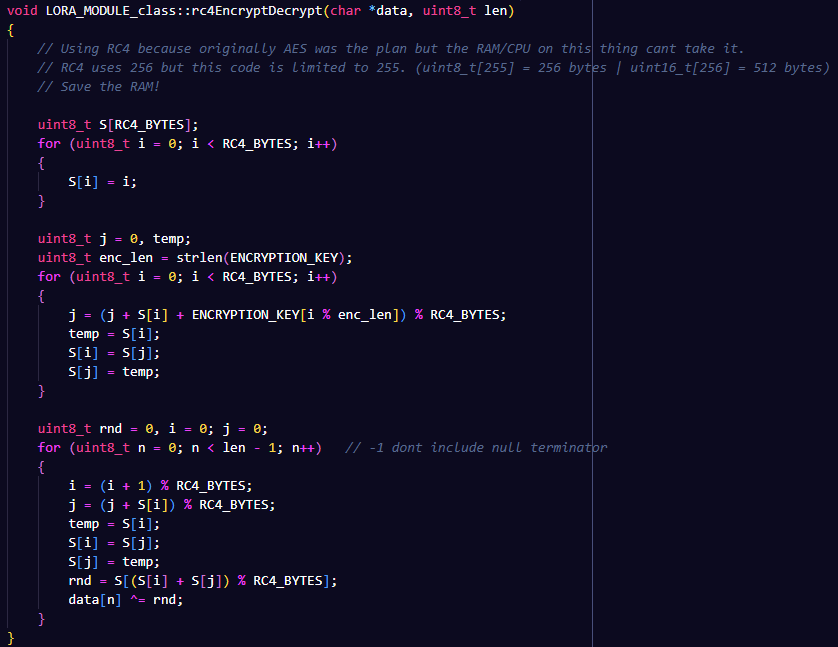
\includegraphics[width=\textwidth,height=5.01875in,keepaspectratio]{figs/method-image10.png}
\end{figure}

\textless talk about the picture here more\textgreater{}

\subsubsection{Mesh Network}

Once a ledger is transmitted, any node within range can receive it,
provided that it is properly formatted. Upon reception, the node
decrypts the packet, extracts the data, and compares it with its local
database. The node then updates its local database using the data from
the received ledger and updates the ledger using its own stored data.
After updating, the ledger may be relayed to other nodes to allow them
to update their respective databases. This process continues until all
nodes possess a fully updated ledger.

Relaying is not automatically performed for every received packet. If
unconditional relaying were implemented, the mesh network would fall
into an infinite rebroadcast loop. Before relaying a ledger, the node
must determine whether retransmission is necessary. If a node receives a
ledger that differs from its local database, it indicates that at least
one node in the network is missing data. In this case, the receiving
node updates the ledger using its local database and relays it, ensuring
that the node which originally transmitted the incomplete ledger
eventually receives the updated information.

For example, if Node 3 receives a ledger that does not contain data from
Node 3, it can infer that somewhere in the network there exists a node
that does not have Node 3's data. Node 3 then updates the ledger and
relays it. This mechanism is not limited to the node's own data. If Node
3 receives a ledger missing Node 5's data, but Node 3 already has Node
5's data stored locally from a previous transmission, Node 3 can update
the ledger and retransmit it. This eliminates the need for the data to
travel multiple hops back to Node 5 before being redistributed,
improving overall efficiency.

The only situation in which a node does not relay a ledger is when the
received ledger is identical to its local database. In this case, all
participating nodes already possess the same data, and retransmission
would only create unnecessary traffic and potential infinite looping.
Therefore, the packet is ignored.

\begin{figure}[htbp]
\centering
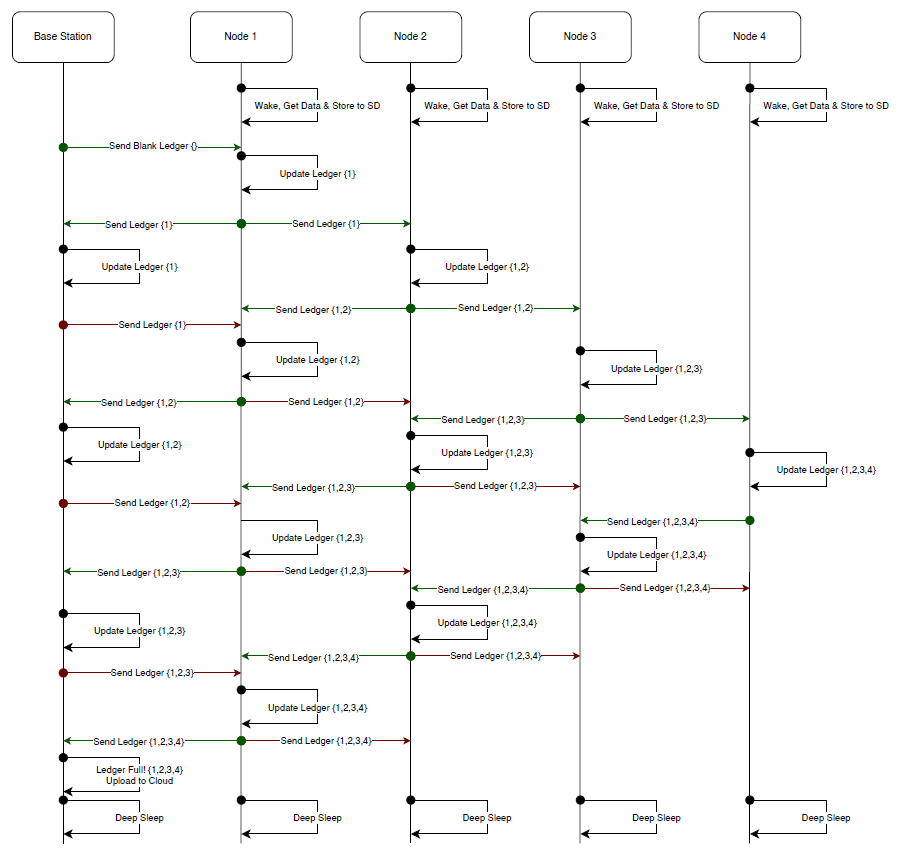
\includegraphics[width=4.43591in,height=4.23923in]{figs/method-image11.png}
\end{figure}

In a linear topology scenario, the base station may only be within range
of Node 1; Node 1 within range of the base station and Node 2; Node 2
within range of Node 1 and Node 3; and so forth. When the base station
sends a packet, Node 1 receives it, updates the ledger, and retransmits
it to nodes within range. This creates a chain reaction until the last
node updates the ledger. The fully updated ledger then propagates back
toward the base station through another chain reaction. Once the base
station receives the complete ledger, the data is saved and uploaded to
the cloud.

\subsubsection{Dealing with Collisions (CSMA/CA (Carrier Sense Multiple Access with Collision Avoidance))}


To prevent simultaneous transmissions that may cause packet collisions,
Carrier Sense Multiple Access with Collision Avoidance (CSMA/CA) is
implemented. Since the LoRa module cannot transmit and receive at the
same time, collision avoidance is necessary to ensure reliable
communication.

Before transmitting, a node first checks the LoRa channel noise level.
If the channel is busy, indicating that packets are currently being
transmitted, the node waits until the channel becomes idle before
attempting to send. This reduces the probability of collision.

However, a node cannot wait indefinitely. Therefore, a timeout mechanism
is implemented. If all nodes were assigned identical timeout values,
collisions could still occur when timeouts expire simultaneously. To
avoid this, each node multiplies the base timeout value by its hardware
ID. This ensures that each node has a different timeout duration. In the
worst-case scenario where all nodes intend to transmit and reach their
timeout, transmissions will occur at different times due to the hardware
ID multiplier.

Additionally, if a node receives a valid packet while waiting to
transmit, it reevaluates the received packet, updates or discards it
accordingly, and restarts its timeout counter. This effectively delays
its transmission and reduces the likelihood of congestion. This
mechanism ensures that channel noise decreases before additional packets
are introduced.

\begin{figure}[htbp]
\centering
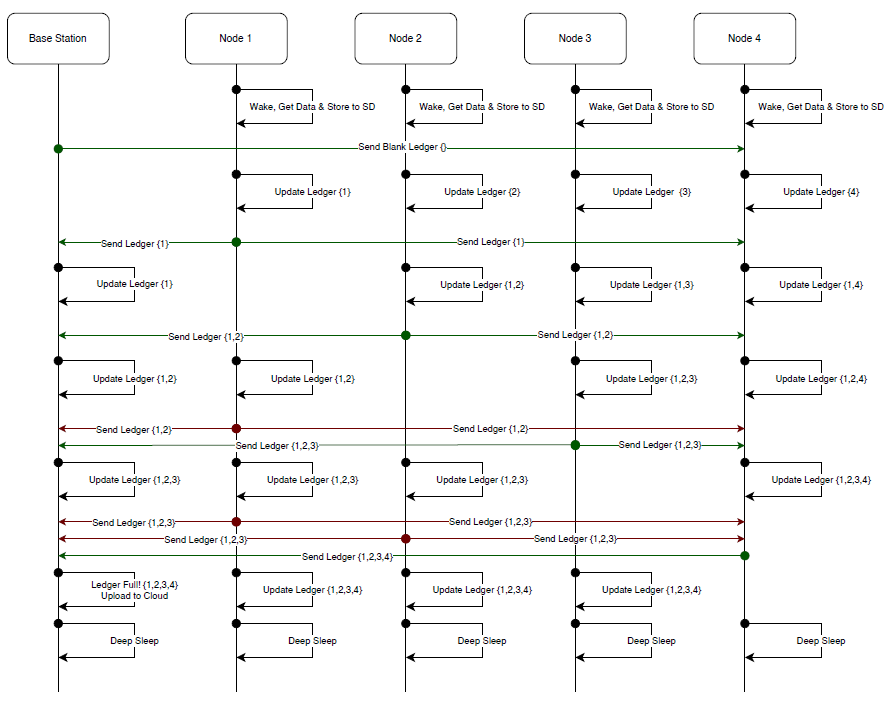
\includegraphics[width=\textwidth,height=5.16528in,keepaspectratio]{figs/method-image12.png}
\end{figure}

In a scenario where all nodes are within range of each other, meaning a
single transmission is received by all nodes, those with lower hardware
IDs transmit first due to shorter timeouts. For example, once all nodes
update their local databases, Node 1 (with the lowest ID) transmits
first. Upon receiving Node 1's transmission, all other nodes stop their
pending transmissions, update their databases, and restart their timeout
process. This continues sequentially until all nodes have shared their
data and the base station receives the complete dataset for upload to
the cloud.

Although this collision avoidance mechanism significantly reduces packet
collisions, it is not perfect. There may be rare timing conditions where
two nodes synchronize unintentionally and transmit simultaneously.
However, due to the mesh structure of the network, the loss of a single
packet is recoverable. Since data is continuously relayed among nodes,
missed information can be recovered from neighboring nodes in subsequent
transmissions.

3.x.x.x.x Lora Firmware Settings (legal standards)

\begin{figure}[htbp]
\centering
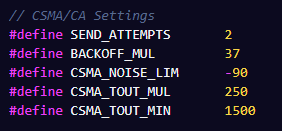
\includegraphics[width=2.93791in,height=1.36477in]{figs/method-image13.png}
\end{figure}

\textless talk about settings here and why they were chosen and legal
limits of how much sending is allowed\textgreater{}

\subsection{In Situ Sensor Behavior and
Algorithm}

The in situ node operates in a low-power duty cycle. It enters deep
sleep mode, wakes up using an RTC timer, gathers sensor data, transmits
data to the mesh network, and then returns to deep sleep. This cycle
repeats continuously throughout
deployment.\begin{figure}[htbp]
\centering
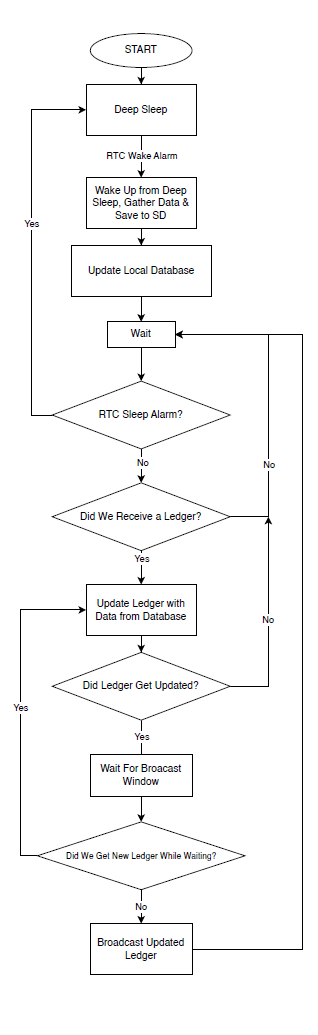
\includegraphics[width=1.36654in,height=4.44873in]{figs/method-image14.png}
\end{figure}

\subsubsection{Sensor Data Reading}

The in situ node contains multiple sensors as previously described: air
temperature and humidity, soil temperature, soil moisture, and battery
voltage. These sensors communicate using different interfaces including
I2C, 1-Wire serial, and analog-to-digital conversion (ADC).

3.4.2.1.1.Air temperature and humidity (aht10)

The AHT10 sensor communicates using the I2C protocol. The
microcontroller sends a measurement command to the sensor, after which
the sensor internally performs the necessary signal processing and
calibration. The processed temperature and humidity data are then
transmitted digitally over the I2C bus to the microcontroller. This
simplifies firmware implementation, as the sensor provides calibrated
digital output directly.

3.4.2.1.2 soil temperature

The DS18B20 soil temperature sensor communicates using the 1-Wire
protocol. Each sensor contains a unique address, allowing individual
identification if multiple sensors share the same bus. The
microcontroller initiates a temperature conversion command and reads the
digital temperature value directly from the sensor, eliminating the need
for analog calibration.

3.4.2.1.3 soil moisture

The soil moisture sensor operates on a capacitive principle. Using a
comparator-based circuit (\_\_\_ chip model), the dielectric constant of
the soil affects the sensor output voltage.

With a 3.3 V supply input, the sensor outputs an analog voltage
proportional to soil moisture. This voltage is read using the 10-bit ADC
of the ATmega328P.

ADC resolution:

\[\text{Resolution} = \frac{V_{ref}}{2^{10}} = \frac{3.3V}{1024}
\]

The raw ADC value is converted to soil moisture percentage using
calibration data obtained through the gravimetric method (see Chapter
\_\_\_).

3.4.2.1.4 battery voltage

The battery voltage is measured using a voltage divider consisting of:

\begin{itemize}
\item
  \(R_{1} = 10\text{ }k\Omega\)
\item
  \(R_{2} = 33\text{ }k\Omega\)
\end{itemize}

Voltage divider formula:

\[V_{out} = V_{battery} \times \frac{R_{2}}{R_{1} + R_{2}}
\]

Rearranged to calculate battery voltage:

\[V_{battery} = V_{ADC} \times \frac{R_{1} + R_{2}}{R_{2}}
\]

The ADC is 10-bit resolution. The digital value is converted to voltage
using the reference voltage and the equation above.

\subsection{Base Station Module
Program}

The base station module operates similarly in low-power mode. It enters
deep sleep and periodically wakes to query the global time from the
internet using pool.ntp.org. When scheduled, it transmits a blank ledger
to initiate mesh data collection. It then waits until it receives a
fully updated ledger containing data from all nodes. Once all required
data has been gathered, it uploads the information to the cloud.

After successful data collection, the base station synchronizes all
nodes by sending a formatted packet containing the correct time obtained
from pool.ntp.org. Although nodes are equipped with RTC modules,
periodic synchronization ensures that all nodes remain aligned and wake
simultaneously, preventing missed data requests.

\begin{figure}[htbp]
\centering
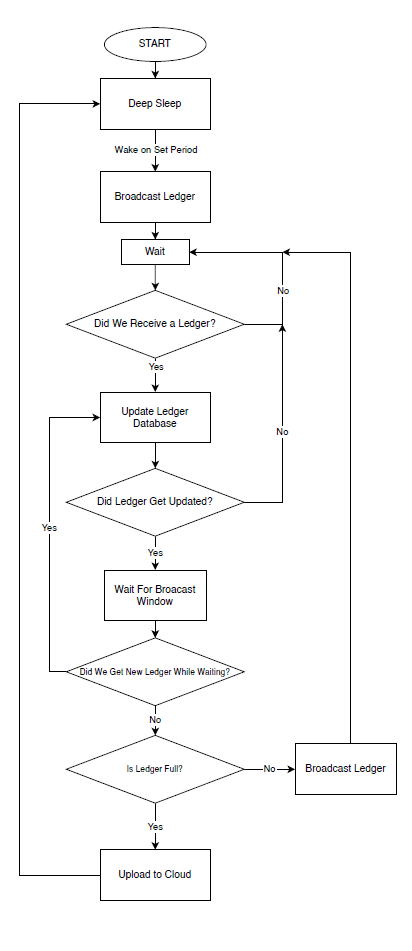
\includegraphics[width=1.41462in,height=3.26566in]{figs/method-image15.png}
\end{figure}

\subsubsection{Uploading the Data}

The cloud platform selected for this project is ThingSpeak.
To upload data, the base station performs an HTTP request using the
ThingSpeak API key. The request is sent using POST/GET (specify which
one is used). Upon successful upload, the server returns status code
\_\_\_.


Since the system can support up to 8 nodes, the base station
uploads each node's data individually using their respective API
keys.


\section{\texorpdfstring{Cloud}{Cloud}}

A cloud-based platform was required to allow researchers to access
sensor data remotely, as the turf houses are located far from the
research facilities and frequent on-site visits are impractical. Storing
data in the cloud enables continuous monitoring and simplifies data
access, making it easier for researchers to view and analyze
measurements without physically retrieving the devices.

Several criteria were considered when selecting a suitable cloud
platform. These included reliability, accessibility, low cost, ease of
integration with embedded systems, and the ability to store and
visualize time-series sensor data. While more advanced platforms such as
AWS or Microsoft Azure provide robust infrastructure, they were
considered unnecessarily complex and costly for the scope of this
project.

Based on these criteria, ThingSpeak was selected as the cloud platform.
ThingSpeak provides reliable data storage and built-in visualization
tools that are well suited for IoT applications. Given the expected data
transmission rate of the system, the required storage and upload
frequency fall within the limits of the free service tier, making it a
cost-effective solution. In this implementation, sensor data uploaded to
the cloud is stored and made readily accessible for remote viewing and
further analysis by researchers.

\section{Testing}

During the development of the project, multiple tests were conducted to
evaluate system performance and reliability. These tests included power
consumption measurements, LoRa range testing, and several preliminary
tests carried out at Háskóli Íslands prior to the final deployment. The
testing phase provided valuable insights into early system limitations
and failures, allowing necessary modifications and improvements to be
made before final deployment.

\subsection{In Situ Sensor Node Power Consumption
Tests}

After the initial assembly of a functional sensor node, power
consumption testing was conducted using a precision laboratory power
supply (Rohde \& Schwarz HMP2030), capable of measuring current down to
100 µA. The sensor module was powered at 4.2 V to represent a fully
charged battery condition, and the power supply's current readout was
used to observe and record current consumption.

During testing, the sensor node was programmed to cycle through multiple
operating states in a continuous loop. Each state was maintained for 10
seconds before transitioning to the next state, allowing the current
readings to stabilize. State transitions were controlled entirely
through firmware to ensure consistent and repeatable behavior. The
measurement cycle was allowed to run continuously, and power consumption
was observed over three complete loops to verify repeatability.

The operating states tested included the following:

\begin{itemize}
\item
  \textbf{Deep sleep mode}
\item
  \textbf{Awake mode with sensors enabled}
\item
  \textbf{LoRa transmission and reception mode}
\item
  \textbf{Half-sleep mode}, in which the sensor modules were
  disconnected while the LoRa module remained fully powered and the MCU
  in a light sleep mode.
\end{itemize}

\textbf{Deep Sleep Mode:}

Deep sleep mode completely shuts down most of the node's hardware
components to minimize power consumption for long-term operation. In
this mode, the system disables communication interfaces such as SPI and
I²C, turns off GPIO modules and the LoRa radio, and sets all pins to a
low-power state. Interrupts from the LoRa module are removed, and only
the real-time clock (RTC) interrupt is enabled to wake the device at
scheduled intervals. The microcontroller then enters the gotosleep()
state where almost all processes are halted. When the RTC interrupt
occurs, the system wakes up, re-enables the LoRa interrupt, powers the
modules back on, and reinitializes the LoRa configuration before
resuming normal operation. This mode is designed to achieve maximum
energy savings for battery-powered wireless sensor nodes that operate
for long periods between transmissions.

\textbf{Light Sleep Mode:}

Light sleep mode reduces power consumption while still keeping certain
communication capabilities active, particularly the LoRa module for
receiving data. In this mode, only non-essential devices and GPIO
modules are powered down, while LoRa is kept in receive mode so the node
can wake immediately when a packet arrives. The I²C communication is
disabled and unused pins are set to low-power states, but the system
maintains the LoRa interrupt to trigger wake-up. When the interrupt from
the LoRa module is detected, the microcontroller exits the sleep state
and resumes execution. Compared to deep sleep, light sleep consumes more
power but allows faster response times and continuous listening for
incoming LoRa messages, making it suitable for nodes that must remain
partially active within the wireless sensor network.

\subsection{Háskóli Íslands Preliminary Tests
1}

After all system components had been assembled and verified, an initial
set of local preliminary tests was conducted at Háskóli Íslands. With
permission from \textbf{{[}NAME TO BE UPDATED{]}} and Dorotea, testing
was carried out on the turf roofs located within the university campus.

A single LoRa base station was installed in Helgi's office, where it was
connected to a computer configured for continuous monitoring of incoming
data via the cloud platform. This setup allowed real-time observation of
device status, packet reception, and data integrity throughout the test
period.

Four sensor devices were deployed across the surrounding area, primarily
in the vicinity of the VR-II and VR-III buildings. All devices were
positioned within an approximate radius of 100 meters from the base
station, ensuring stable connectivity while enabling early validation of
system reliability under realistic deployment conditions. For this test,
each sensor was powered by a single battery cell in order to evaluate
power consumption and determine the operational lifetime achievable with
one cell.

The preliminary test phase was conducted over a three-week period, from
\textbf{June 8 to June 29, 2025}. During this time, the system operated
continuously, providing insight into long-term stability, data
consistency, and potential environmental effects on communication
performance.

\subsection{LoRa Range Tests}

Based on insights gained from the initial field tests, it became
necessary to conduct more extensive range testing to further evaluate
system performance under different conditions. Multiple LoRa
configurations were evaluated to determine the most optimal balance
between communication range and performance. Previous studies have
demonstrated that LoRa is capable of achieving significant transmission
distances under suitable conditions, and these claims needed to be
validated using the current hardware setup and deployment environment.

The LoRa transceiver supports a wide range of configurable parameters,
including operating frequency, transmission power, bandwidth, sync word,
spreading factor, coding rate, and preamble length. For these
experiments, several of these parameters were kept constant---namely
frequency, transmission power, sync word, coding rate, and preamble
length---in order to ensure fair and repeatable comparisons between
tests. The parameters that were primarily adjusted during testing were
bandwidth and spreading factor, as these have the most direct and
significant impact on range, data rate, and signal robustness.

\textbf{Key LoRa configuration parameters:}

\begin{itemize}
\item
  \textbf{Bandwidth (BW):} Determines the width of the frequency band
  used for transmission. Lower bandwidth improves receiver sensitivity
  and increases range, but reduces data rate.
\item
  \textbf{Spreading Factor (SF):} Controls how many chirps are used to
  encode each symbol. Higher spreading factors increase range and
  resistance to noise at the cost of lower data rates and longer
  transmission times.
\item
  \textbf{Transmission Power:} Defines the output power of the radio.
  This was kept constant to comply with regulatory limits and to isolate
  the effects of BW and SF.
\item
  \textbf{Coding Rate (CR):} Adds forward error correction to improve
  data reliability. This was fixed to maintain consistent error
  correction across tests.
\item
  \textbf{Preamble Length:} Used for receiver synchronization. A fixed
  preamble ensured consistent packet detection behavior.
\end{itemize}

Bandwidth and spreading factor were the primary variables during testing
because together they directly influence link budget and receiver
sensitivity. Adjusting other parameters would either violate regulatory
constraints or introduce additional variables that make performance
comparisons less reliable. By focusing on BW and SF, it was possible to
observe clear trade-offs between range, signal quality, and data
throughput.

The range tests were conducted in Vellir, located in Hafnarfjörður. The
base station was mounted on a fence at approximately chest height to
simulate a realistic low-elevation deployment. A mobile sensor node was
placed inside a vehicle and connected to a laptop for real-time
monitoring.

During the tests, the vehicle was driven around the surrounding area
while the base station transmitted randomly encoded data packets once
per second. The received signal strength indicator (RSSI) values were
recorded continuously, and received packets were inspected to verify
data integrity and detect any corruption. This approach allowed both
communication reliability and signal strength to be evaluated
simultaneously under real-world conditions.

\subsection{Háskóli Íslands Preliminary Tests
2}

Building on the insights gained from the previous preliminary tests and
subsequent system improvements, a longer-duration local test was
conducted at Háskóli Íslands. Due to seasonal conditions approaching
winter, access to the turf roofs was no longer permitted, as they were
required for ongoing studies by the responsible staff member.

As a result, four sensor devices were redeployed across the campus
within an approximate radius of 100 meters from the base station, using
the same monitoring and data collection setup as in the earlier tests.
The base station remained connected to a dedicated computer for
continuous cloud-based data monitoring. In this test, each sensor was
powered by a single battery cell, consistent with the previous test
configuration.

For this test phase, the antenna system was upgraded to improve
communication performance. Larger and higher-quality antennas were
installed on the sensor nodes, and an outdoor antenna was mounted
outside Helgi's office to enhance base station reception and
transmission.

This second preliminary test was conducted over an extended period, from
\textbf{August 1 to October 6, 2025}, allowing for evaluation of
long-term system stability, communication reliability, and the impact of
environmental conditions on performance.

\section{Deployment in Keldur}

After incorporating lessons learned from the previous test phases, the
system was considered ready for full deployment. In collaboration with
Dorotea, a deployment visit was arranged to \textbf{Keldur} (additional
site information to be added).

For this deployment, each sensor node was configured with the maximum
number of battery cells supported by the enclosure, which was three
cells per sensor. All sensors were fully sealed and prepared for
long-term outdoor operation prior to deployment.

Upon arrival at Keldur, the network infrastructure was already in place
from earlier testing. The Wi-Fi router was located in the attic of one
of the turf houses. The LoRa base station was installed at this location
and connected to the existing network, allowing immediate communication
with the cloud platform. Once verified, the base station equipment was
discreetly concealed to avoid visual impact, as the site operates as a
museum.

Following the base station setup, four sensor units were installed
around the area, with one sensor assigned to each turf roof.

\emph{{[}Further details describing sensor placement, mounting method,
and orientation to be added here, along with reference to deployment
photographs.{]}}

After installation, all equipment was confirmed to be operational and
securely concealed. The long-term deployment test commenced on
\textbf{October 17, 2025}, and is currently ongoing \textbf{{[}end date
to be updated upon completion{]}}.

\section{Calibration Method}

To determine the accuracy of the off-the-shelf soil moisture sensors
relative to an industry-standard instrument, the sensors were compared
side by side with a HOBO MX230x Soil Moisture and Temperature Data
Logger. The HOBO device is a fully integrated soil moisture logger with
Bluetooth-based wireless data offload capability and measures both soil
moisture and temperature.

To ensure scientific accuracy, the gravimetric method was performed
alongside the sensor comparison to establish the actual soil moisture
content. Calibration was conducted at {[}insert laboratory name{]}
located at VR-3.

An Icelandic soil sample was collected and oven-dried at 105 °C for 32
hours (from 11:00 AM to 8:00 PM the following day) to remove all
moisture and establish a dry baseline condition. After drying, the soil
was allowed to cool to room temperature before testing. A measured
portion of the dried soil was then placed in a container, and all
sensors were installed side by side to ensure identical environmental
conditions.

Water was added incrementally in 10\% increments relative to the dry
soil weight. A spray mister was used to distribute water evenly
throughout the soil. After each increment, sufficient time was allowed
for uniform saturation before measurements were recorded. At each
moisture level, multiple readings were collected from all sensors to
ensure consistency and reduce variability. This procedure was repeated
for each incremental moisture level.

The HOBO sensor provides measurements of volumetric water content (VWC)
in mineral soils, with a specified measurement range of 0.00 to 0.64
m³/m³. In this experiment, mineral soil configuration was used. Although
the device also allows alternative output settings, the selected
configuration was kept consistent throughout the experiment. Where
necessary, conversion equations were applied during data analysis to
ensure comparability of results.

The experiment continued until the soil reached full saturation and
additional water resulted in surface pooling, indicating that no further
absorption could occur. At this point, the calibration process was
concluded and all measurements were recorded and stored for analysis.

To ensure reliability and repeatability, the entire calibration
procedure was conducted twice. The first experiment was performed on
November 8, and the second on December 16.

\textbf{3.8.1 Reference Instrument: HOBO MX230x Soil Moisture and
Temperature Data Logger}

The HOBO MX230x Soil Moisture and Temperature Data Logger was used as
the reference instrument for calibration. This commercial device is
widely used in environmental monitoring studies and is also currently
utilized by research teams working on Icelandic turf roof monitoring.
Using this instrument as the reference ensures consistency and
comparability with existing research efforts.

The soil moisture sensor measures volumetric water content (VWC) with a
measurement range of 0.00 to 0.64 m³/m³ in mineral soils and 0.00 to
0.70 m³/m³ in soilless media. The typical accuracy is ±0.031 m³/m³ in
mineral soils (solution EC \textless{} 8 dS/m), with a resolution of
0.001 m³/m³. The sensor operates at a dielectric measurement frequency
of 70 MHz.

The integrated temperature sensor (MX2307) has a measurement range of
−40 °C to 100 °C with an accuracy of ±0.2 °C to ±0.25 °C depending on
the temperature range, and a resolution of 0.04 °C. The logger supports
adjustable logging intervals from 1 second to 18 hours and can store up
to 110,000 measurements. The device uses Bluetooth Low Energy for
wireless data retrieval and is powered by a 3.6 V lithium battery with a
typical operational life of up to several years, depending on logging
configuration.

The manufacturer also specifies that the soil moisture measurements can
be post-calibrated using custom calibration equations if higher accuracy
is required or if soil conditions differ from standard mineral soils.
This feature further supports its suitability as a calibration reference
instrument for this study.
